
% Nature Communications:
% The main text (not including abstract, Methods, References and figure legends) is limited to 5,000 words. The maximum title length is 15 words. The abstract — which should be no more than 150 words long and contain no references — should serve both as a general introduction to the topic and as a brief, non-technical summary of the main results and their implications.

% The main text of an Article should begin with an introduction (without heading) of referenced text that expands on the background of the work (some overlap with the abstract is acceptable), followed by sections headed Results, Discussion (if appropriate) and Methods (if appropriate). The Results and Methods sections may be divided by topical subheadings; the Discussion should be succinct and may not contain subheadings. Figure legends are limited to 350 words each. References are limited to 70. Footnotes are not used.

% Depending on the word count, Articles may have up to 10 display items (figures and/or tables). In addition, a limited number of uncaptioned molecular structure graphics and numbered mathematical equations may be included if necessary. To enable typesetting of papers, the number of display items should be commensurate with the word length — those with word counts less than 2,000 should have no more than 4 figures/tables. Please note that schemes are not used; these should be presented as figures.

% Current Biology:
% Articles present conceptual advances of unusual significance regarding a biological question of wide interest. Articles are typically limited to ten journal pages (usually around 5000 words of main text, i.e. all of the text in the manuscript except for the summary, references, and any Supplemental Information text), and there should be no more than seven display items (figures and tables). Additional items and details may be published online as Supplemental Information at the discretion of the editor (please see the Supplemental Information guidelines for more information).

% TG: Good thing is that it's the same format for both!

%%%%%%%%%%%%%%%%%%%%%%%%%%%%%%%%%%%%
% SHORTENED REARANGED VERSION
%
% The tag % RM is for simply removing the line
% The tag % TO-SUP is to move the part to the supplementary
%%%%%%%%%%%%%%%%%%%%%%%%%%%%%%%%%%%%


\documentclass[12pt,letterpaper]{article}


%Packages
\usepackage{pdflscape}
\usepackage{fixltx2e}
\usepackage{textcomp}
\usepackage{fullpage}
\usepackage{float}
\usepackage{latexsym}
\usepackage{url}
\usepackage{epsfig}
\usepackage{graphicx}
\usepackage{amssymb}
\usepackage{amsmath}
\usepackage{bm}
\usepackage{array}
\usepackage[version=3]{mhchem}
\usepackage{ifthen}
\usepackage{caption}
\usepackage{hyperref}
\usepackage{amsthm}
\usepackage{amstext}
\usepackage{enumerate}
\usepackage[osf]{mathpazo}
\usepackage{dcolumn}
\usepackage{lineno}
\usepackage{dcolumn}
\usepackage{filecontents}

\newcolumntype{d}[1]{D{.}{.}{#1}}

\pagenumbering{arabic}


%Pagination style and stuff
\linespread{2}
\raggedright
\setlength{\parindent}{0.5in}
\setcounter{secnumdepth}{0} 
\renewcommand{\section}[1]{%
\bigskip
\begin{center}
\begin{Large}
\normalfont\scshape #1
\medskip
\end{Large}
\end{center}}
\renewcommand{\subsection}[1]{%
\bigskip
\begin{center}
\begin{large}
\normalfont\itshape #1
\end{large}
\end{center}}
\renewcommand{\subsubsection}[1]{%
\vspace{2ex}
\noindent
\textit{#1.}---}
\renewcommand{\tableofcontents}{}
%\bibpunct{(}{)}{;}{a}{}{,}

%---------------------------------------------
%
%       START
%
%---------------------------------------------

\begin{document}

%Running head
\begin{flushright}
Version dated: \today
\end{flushright}
\bigskip
%\noindent RH: No effect of the K-Pg event on mammal disparity.

\bigskip
\medskip
\begin{center}

%Title 15 words max
\noindent{\Large \bf Mammalian morphological diversity does not increase in response to the Cretaceous-Paleogene mass extinction.}% and the extinction of the (non-avian) dinosaurs.} 
\bigskip 

\noindent {\normalsize \sc Thomas Guillerme$^1$$^,$$^*$, and Natalie Cooper$^2$}\\
\noindent {\small \it 
$^1$School of Natural Sciences, Trinity College Dublin, Dublin 2, Ireland.\\
$^2$Department of Life Sciences, Natural History Museum, Cromwell Road, London, SW7 5BD, UK.}\\
\end{center}
\medskip
\noindent{*\bf Corresponding author.} \textit{guillert@tcd.ie}\\  
\vspace{1in}

%Line numbering
\modulolinenumbers[1]
\linenumbers

%---------------------------------------------
%
%       ABSTRACT
%
%---------------------------------------------

\newpage
\begin{abstract}
% TG: this must be reduced to 150 words
% Popular science accounts state that after the extinction of the non-avian dinosaurs at the Cretaceous-Paleogene (K-Pg) boundary 66 million years ago, mammals rapidly diversified to fill their empty ecological niches.
% However, evidence for this is mixed. 
% Palaeontological analyses suggest that mammals radiated in response to the K-Pg extinction event, whereas neontological analyses suggest that mammals began to radiate before K-Pg and were not greatly affected by it. 
% Here we aim to end this debate by looking at living and fossil taxa simultaneously.

% We investigated the effect of the K-Pg extinction event on mammalian morphological diversity (disparity) using two Total Evidence tip-dated phylogenies of Mammaliaformes and Eutheria, containing both living and fossil taxa. 
% Using a novel, continuous time-slicing method for measuring changes in disparity-through-time, we found no significant change in disparity before and after the K-Pg boundary, under either a gradual or punctuated model of evolution.
% This implies that the extinctions at the end of the Cretaceous did not affect mammalian morphological evolution. 
% Our findings contradict the popular theory that the non-avian dinosaurs and other Mesozoic tetrapods were restricting mammalian evolution, and that their extinction liberated ecological niches for mammals to evolve into.

% TG: shortened version (150 words sharp!)
Popular science accounts state that after the extinction of the non-avian dinosaurs at the Cretaceous-Paleogene (K-Pg) boundary 66 million years ago, mammals rapidly diversified to fill their empty ecological niches.
However, evidence for this is mixed. 
Palaeontological data suggest that mammals radiated in response to the K-Pg event, whereas neontological data suggest that they were not really affected by it.
Here we aim to end this debate by looking at both data simultaneously.

We investigated the effect of the K-Pg event on mammalian morphological diversity (disparity) using two Total Evidence tip-dated phylogenies of Mammaliaformes and Eutheria, containing both living and fossil taxa. 
Using a novel, continuous time-slicing method for measuring changes in disparity-through-time, we found no significant change in disparity before and after the K-Pg boundary.
Our findings contradict the popular theory that non-avian dinosaurs were restricting mammalian evolution, and that their extinction liberated ecological niches for mammals to evolve into.

\end{abstract}

\noindent (Keywords: disparity, punctuated equilibrium, gradual evolution, time slicing, K-Pg)\\

\vspace{1.5in}

\newpage 

%---------------------------------------------
%
%       INTRODUCTION
%
%---------------------------------------------

\section{Introduction}
Throughout history, life on Earth has suffered a series of mass extinction events resulting in drastic declines in global biodiversity (e.g. \cite{RaupPT,BentonPT,rennetime2013,Brusatte2015}).
The long-term effects of mass extinctions, however, are more varied \cite{Erwin1998344}, and include species richness increases in some clades \cite{friedmanexplosive2010} and declines in others \cite{Brusatte2015}
, changes in morphological diversity \cite{kornextinction2013} and shifts in ecological dominance (e.g. \cite{Brusatte12092008,toljagictriassic-jurassic2013,bensonfaunal2014}).
These shifts are characterised by the decline of one clade that is replaced by a different unrelated clade with a similar ecological role (e.g. Brachiopoda and Bivalvia at the end Permian extinction; \cite{Liow2015}).
Shifts in ecological dominance are of particular interest because they are a fairly common pattern observed in the fossil record (e.g. Foraminifera; \cite{Coxall01042006}; Ichtyosauria; \cite{thorneresetting2011}; Plesiosauria; \cite{bensonfaunal2014}) and are often linked to major macroevolutionary processes such as adaptive \cite{Losos2010} or competitive \cite{Brusatte12092008} radiations.

One classical example of a shift in ecological dominance is at the Cretaceous-Palaeogene (K-Pg) mass extinction 66 million years ago (Ma) \cite{rennetime2013}, where many terrestrial vertebrates (including the dominant non-avian dinosaur group; \cite{archibald2011extinction,rennetime2013,Brusatte2015}) went extinct, allowing placental mammals to dominate the fauna \cite{archibald2011extinction,Lovergrove}. 
Some authors suggest this reflects placental mammals filling the ``empty'' niches left after the K-Pg extinction event \cite{archibald2011extinction,OLeary08022013}, others suggest it reflects a release from predation and/or competition \cite{Slater2012MEE,Lovergrove}.
However, evidence for the diversification of placental mammals being driven by the K-Pg extinction event is mixed.
Thorough analysis of the fossil record (e.g. \cite{goswamia2011,OLeary08022013}) supports the idea that placental mammals diversified after the K-Pg extinction event as there are no undebated placental mammal fossils before it and many afterwards \cite{archibald2011extinction,goswamia2011,Slater2012MEE,OLeary08022013,Wilson2013,Brusatte2015}. 
Conversely, evidence from molecular data suggests that the diversification of placental mammals started prior to the K-Pg extinction event without being drastically affected by it (e.g. \cite{bininda2007delayed,meredithimpacts2011,Stadler12042011}).
Therefore, whether the diversification of placental mammals began before the K-Pg extinction event, or in response to the extinctions at K-Pg, is a matter of great debate \cite{dosReis2012,OLeary08022013,Springer09082013,OLeary09082013,dosReis2014}. 

There are two main reasons why there is still debate about the timing of the diversification of placental mammals. 
Firstly, palaeontological and neontological data show different patterns; palaeontological data generally suggest that placental mammals diversified after K-Pg (e.g. \cite{OLeary08022013}), whereas neontological data suggest that K-Pg extinction event had little to no effect on mammalian diversification \cite{bininda2007delayed,meredithimpacts2011,Stadler12042011}.
We can solve this issue by using both palaeontological and neontological data in our analyses. 
The Total Evidence method allows us to use cladistic data for both living and fossil taxa, along with molecular data for living taxa, to build phylogenies \cite{ronquista2012}.
This method can also be combined with the tip-dating method \cite{ronquista2012} to get more accurate estimates of diversification times for both living and fossil species.
Here we use two recent Total Evidence tip-dated phylogenies of mammals \cite{Slater2012MEE,beckancient2014} to investigate palaeontological and neontological taxa simultaneously.

A second issue is that diversity can be defined in many different ways.
In many studies it is measured as taxonomic diversity or species richness \cite{Stadler12042011,meredithimpacts2011,OLeary08022013}, but often the more interesting aspect of diversity is related to the ecological niches the species occupy \cite{Brusatte12092008,toljagictriassic-jurassic2013}, particularly if we want to make hypotheses about macroevolutionary processes \cite{Losos2010,glor2010phylogenetic,benton2015}.
Sometimes taxonomic diversity is used as a proxy for other kinds of diversity, however, species richness can be decoupled from morphological diversity (e.g. \cite{slaterCetacean,ruta2013,hopkinsdecoupling2013}), so it may not be the best proxy for ecological diversity.
We can instead use morphological diversity, also known as disparity (e.g. \cite{Wills1994}), as a way to quantify changes in mammalian morphology that should relate to the ecology of the species.
However some methods for measuring disparity are outdated and make inappropriate assumptions.
Many methods for quantifying changes in morphological diversity were proposed $>$ 20 years ago \cite{Foote01071994,Wills1994} and are sometimes used without modifications (e.g. \cite{Brusatte12092008,thorneresetting2011,toljagictriassic-jurassic2013,ruta2013,bensonfaunal2014}).
Additionally, previous methods are based on an underlying assumption that changes in disparity occur by punctuated evolution (e.g. \cite{Brusatte12092008}) which is not always the case \cite{Hunt21042015}.
Finally, most studies of disparity-through-time use unequal time units based on biostratigraphy \cite{Brusatte12092008,toljagictriassic-jurassic2013}. 
This can be tautological as biostratigraphy is already based on changes in fossil assemblages and morphology through time.
To deal with these issues, we propose an updated approach to test whether mammals diversified in response to the K-Pg event, using morphological disparity, measured as cladistic disparity (see Methods), as our proxy for diversity.

Here we measure the disparity of living and fossil mammals before or after K-Pg, using cladistic morphological matrices and Total Evidence tip-dated trees taken from two previous studies on Mammaliaformes (family-level, 103 taxa, 446 morphological characters, 310 Ma to present \cite{Slater2012MEE}) and Eutheria (genus-level, 102 taxa, 421 morphological characters, 170 Ma to present \cite{beckancient2014}). 
Using a novel time-slicing approach, we produce fine-grained estimates of disparity-through-time under two different models of morphological character evolution (either gradual or punctuated). 
We also test whether mammals display significant changes in disparity between the end of the Cretaceous and throughout the Cenozoic.
Until now, this question has only been investigated using data from North American Therian mammals (excluding Monotremata) and without formally testing the effect of the K-Pg extinction event \cite{Wilson2013}.
To our knowledge, this study is the first to approach the debate about the effects of the K-Pg extinction event on mammalian evolution using Total Evidence phylogenies and by calculating disparity-through-time in a continuous way.


%---------------------------------------------
%
%       RESULTS
%
%---------------------------------------------

\section{Results}
Disparity in the Mammaliaformes reaches a plateau during the Middle Triassic around 240 Ma, and fluctuates slightly around this during the rest of the Mesozoic and the Cenozoic (Fig \ref{fig:Fig_Raw_results} and Fig S5).
In the Eutheria, disparity reaches a plateau at the end of the Jurassic around 150 Ma.
These patterns are similar whether a gradual or punctuated model of evolution was used to calculate disparity at each time subsample (Fig \ref{fig:Fig_Raw_results}; see Methods).

If the K-Pg extinction event had a significant effect on mammalian disparity, we should see a significant difference between disparity at the end of the Cretaceous and disparity at the start of the Paleogene.
Here, however, we found no significant differences in disparity between the last subsample of the Cretaceous (70 Ma) and the first subsample of the Paleogene (65 Ma; Table \ref{tab:Tab_results}) for either Mammaliaformes or Eutheria, under both gradual and punctuated evolutionary models. 
It is possible that the effect of extinction on a group's evolution might not be detectable directly after the event due to delays in recovery, for example, ecosystems only fully recovered 8-9 Ma after the Permo-Triassic mass extinction \cite{chen2012timing} (although effects on mammalian evolution have been detected as early as 500,000 years after K-Pg \cite{Wilson2013}).
Additionally, some authors argue that the major diversification event in mammals took place during the Paleocene-Eocene Thermal Maximum (PETM; $\sim$ 56 Ma \cite{bininda2007delayed} but see \cite{meredithimpacts2011,Stadler12042011}) with the extinctions at K-Pg providing the ``empty'' ecological space required for this diversification to occur.
We therefore extended our comparisons between the last subsample of the Cretaceous (70 Ma) up to the late Eocene (35 Ma) to check for a delayed effect of the K-Pg extinction potentially allowing morphological diversification after the PETM. 
We also found no significant differences in disparity between the last subsample of the Cretaceous (70 Ma) and any subsamples of the Paleocene and Eocene for Mammaliaformes under both evolutionary models and for Eutheria under a gradual evolutionary model (Table \ref{tab:Tab_results}).
However, in Eutheria under the punctuated evolutionary model, we found a small significant difference (after applying Bonferonni corrections) in disparity between the last subsample of the Cretaceous (70 Ma) and the subsamples at 45 Ma (an increase in disparity of 0.17; Table \ref{tab:Tab_results}).
However, this result is not significant when we control for the number of taxa present in each time subsample (Table S1). 

Changes in disparity may reflect changes in the numbers of taxa represented in each time subsample, with subsamples that have more taxa having higher disparity. 
However, this does not appear to be a problem in our analyses as, for both Mammaliaformes and Eutheria, the same patterns and results are seen in the rarefied analyses (Fig \ref{fig:Fig_Raw_results} and S3; Table S1) where we standardised the number of tips and nodes (a proxy for taxonomic richness) in each time subsample (see Methods).
Additionally, patterns of disparity-through-time and taxon-richness-through-time do not match.
In Mammaliaformes the number of tips and nodes in each time subsample steadily increase until the Middle Jurassic around 170 Ma (Fig S5) then randomly fluctuate during the rest of the Mesozoic and the Cenozoic (Fig \ref{fig:Fig_Raw_results}).
In Eutheria, the number of tips and nodes increases up to the K-Pg boundary and then decreases throughout the Cenozoic (Fig \ref{fig:Fig_Raw_results}).

\begin{figure}[!htbp]
\centering
    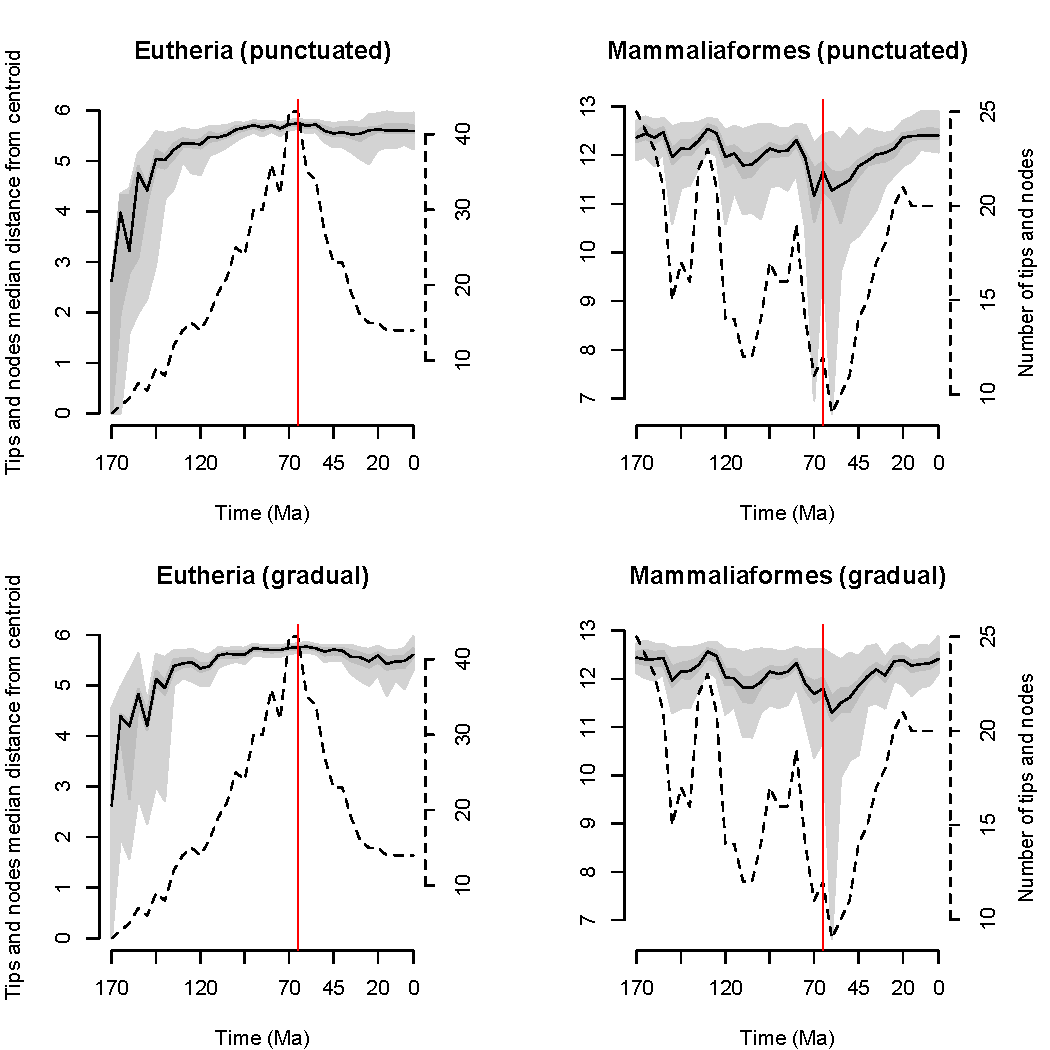
\includegraphics[keepaspectratio=true]{Figures/Main_results.pdf}
\caption{\scriptsize{Disparity-through-time in Eutheria and Mammaliaformes calculated using a model of punctuated (upper panels) or gradual (lower panels) evolution. The x axis represents time in millions of years before the present (Ma). The y axis represents disparity, measured as the median distance between the centroid of the ordinated space and the tips/nodes in each time subsample. The solid black lines show the mean disparity estimated from 1000 bootstrapped pseudoreplicates and confidence intervals (CI) are represented by the grey polygons (50\% CI in dark grey and 95\% CI in light grey). The dashed line and the right hand axis represents the number of tips/nodes in each time subsample. The red vertical line indicates the Cretaceous-Paleogene (K-Pg) boundary (66 Ma). Note that scale bars differ among panels.}}
\label{fig:Fig_Raw_results}
\end{figure}

\begin{table}[ht]
\caption{\scriptsize{Results of \textit{t}-tests comparing disparity at the last subsample of the Cretaceous (70 Ma) to subsamples of the Paleocene and Eocene, under both gradual and punctuated evolutionary models, in Mammaliaformes and Eutheria. Difference = mean difference in disparity between the two subsamples being compared; df = degrees of freedom; p value = original p value prior to Bonferonni correction. Significant differences (after applying Bonferonni corrections for multiple comparisons) are highlighted in bold.}}
\label{tab:Tab_results}
\centering
\begin{tabular}{c|cccc|cccc}
  \hline
  \textbf{Subsamples} & \multicolumn{4}{c|}{\textbf{Gradual evolution model}} & \multicolumn{4}{c}{\textbf{Punctuated evolution model}} \\
  \textbf{compared} & \textbf{difference} & \textbf{df} & \textbf{t} & \textbf{p value} & \textbf{difference} & \textbf{df} & \textbf{t} & \textbf{p value} \\ 
  \hline
  \multicolumn{9}{c}{\textbf{Mammaliaformes}}\\
  \hline
  70 \textit{vs.} 65 & -0.420 & 21 & -0.808 & 0.428 & -0.030 & 21 & -0.058 & 0.954 \\ 
  70 \textit{vs.} 60 & 0.030 & 18 & 0.046 & 0.964 & 0.210 & 18 & 0.379 & 0.709 \\ 
  70 \textit{vs.} 55 & 0.010 & 19 & 0.021 & 0.983 & 0.110 & 19 & 0.225 & 0.824 \\ 
  70 \textit{vs.} 50 & -0.260 & 20 & -0.456 & 0.653 & 0.030 & 20 & 0.060 & 0.953 \\ 
  70 \textit{vs.} 45 & -0.430 & 23 & -0.869 & 0.394 & 0.060 & 23 & 0.132 & 0.896 \\ 
  70 \textit{vs.} 40 & -0.620 & 24 & -1.388 & 0.178 & -0.410 & 24 & -1.031 & 0.313 \\ 
  70 \textit{vs.} 35 & -0.730 & 26 & -1.742 & 0.093 & -0.340 & 26 & -0.861 & 0.397 \\ 
  \hline
  \multicolumn{9}{c}{\textbf{Eutheria}}\\
  \hline
  70 \textit{vs.} 65 & -0.020 & 84 & -0.503 & 0.616 & 0.010 & 84 & 0.288 & 0.774 \\ 
  70 \textit{vs.} 60 & 0.030 & 76 & 0.617 & 0.539 & 0.080 & 76 & 1.693 & 0.095 \\ 
  70 \textit{vs.} 55 & 0.030 & 75 & 0.519 & 0.605 & 0.030 & 75 & 0.699 & 0.486 \\ 
  70 \textit{vs.} 50 & 0.130 & 68 & 2.101 & 0.039$^1$ & 0.080 & 68 & 1.458 & 0.149 \\ 
  70 \textit{vs.} 45 & 0.190 & 64 & 2.679 & 0.009$^1$ & 0.170 & 64 & 2.730 & \textbf{0.006}$^2$ \\ 
  70 \textit{vs.} 40 & 0.160 & 64 & 2.249 & 0.028$^1$ & 0.130 & 64 & 2.084 & 0.041$^1$ \\ 
  70 \textit{vs.} 35 & 0.190 & 60 & 2.358 & 0.022$^1$ & 0.120 & 60 & 1.893 & 0.063 \\ 
   \hline
\end{tabular} \\
   \small{$^1$p value is non-significant after applying Bonferonni correction;
   $^2$p value is \textbf{0.048} after applying Bonferonni correction.}
\end{table}



%---------------------------------------------
%
%       DISCUSSION
%
%---------------------------------------------

\section{Discussion}
% §1 - What did we found
Previous authors have suggested that the K-Pg extinction event released mammals from ecological pressures such as competition and predation, allowing them to radiate into newly available ecological niches \cite{archibald2011extinction,OLeary08022013,Lovergrove,Slater2012MEE}.
However, we did not detect any significant changes in mammalian disparity before and after K-Pg in either Mammaliaformes or Eutheria, under a model of punctuated or gradual evolution.
Additionally, we tested whether the absence of a detectable effect might be due to a lag effect, with the effect only becoming obvious later in the Paleocene.
Even when accounting for such a lag effect, we did not detect any significant effect of the K-Pg extinction event on mammalian disparity.
Our results imply that mammals did not diversify morphologically in response to the K-Pg extinction event.
Instead, their diversification appears to have begun before the end of the Cretaceous (Fig \ref{fig:Fig_Raw_results}, Table \ref{tab:Tab_results} and see \cite{meredithimpacts2011,dosReis2014,Close2015,Lee2015R759}).

% §3 - but PETM story
We did, however, detect a small, yet significant, increase in disparity during the Eocene (45 Ma) under a punctuated evolutionary model using the Eutheria dataset.
This might be due to a long lag effect of $\sim$21 Ma after K-Pg.
Note however, that this is double the lag time observed in other mass extinctions \cite{chen2012timing}.
Therefore, it may be more likely to be attributed to a lag effect of the Palaeocene-Eocene Thermal Maximum (PETM; $\sim$11 Ma afterwards \cite{bininda2007delayed}).
However, this significant increase in disparity is only detected at 45 Ma but not afterwards (which would be expected if the increase was due to an evolutionary radiation) and is not seen under the gradual evolution model.
This indicates that it is more likely due to differences in the evolutionary models rather than an actual increase in disparity.
The 45 Ma subsample samples the long branch ($\sim$50 million years) leading to \textit{Lepidictis} (33.9 to 33.3 Ma) that branches with its closest relative \textit{Gypsonictops} (66.8 to 66 Ma) in the early Upper Cretaceous $\sim$90 Ma (see Fig S2).
Therefore, in this time-subsample under the gradual evolution model, the data for \textit{Lepidictis} is always sampled, but under the punctuated evolution model the algorithm can also randomly sample the data from its ancestor in the early Upper Cretaceous (see methods).
This may inflate differences compared to other subsamples.
Incidentally, this increase can also be linked to the number of tips and nodes used in the comparison (43 versus 23 tips and nodes at respectively 70 and 45 Ma), because the increase is not significant in the rarefied analysis (see Fig S3 with only eight tips and nodes).
Given these caveats we believe that no strong conclusions can be drawn from the increase in disparity during the Eocene.

% §4 - How does that compare to other people
Our results differ from a previous study that found an increase in disparity in North American Theria as soon as $\sim$0.5 Ma after K-Pg \cite{Wilson2013}.
These differences are likely to be related to several methodological differences between the present study and the previous one \cite{Wilson2013}.
Firstly, \cite{Wilson2013} only measures disparity at a regional scale (North America) and proposes that the observed increases in disparity are linked to the immigration of new species into the study localities.
This strongly implies that disparity was higher on a global scale.
Secondly, most of the debate on mammalian diversification around the K-Pg boundary seems to be linked to the conflicting signal between palaeontological and neontological data (\cite{meredithimpacts2011} \textit{vs.} \cite{OLeary08022013} but see \cite{dosReis2014}).
Therefore, an effect of the K-Pg extinction event might be detectable only when using just palaeontological data.
In this study, however, we use Total Evidence tip-dated trees based on both palaeontological and neontological data \cite{Slater2012MEE,beckancient2014}, which may account for the differences between our study and that of \cite{Wilson2013} who used only fossil data.

% §5 - However, our results differ from Slater
Interestingly, however, our results also differ from \cite{Slater2012MEE}, the source of data for the Mammaliaformes dataset.
\cite{Slater2012MEE} found support for a shift in the mode of body mass evolution (from an Ornstein--Uhlenbeck to a Brownian Motion model) directly after K-Pg suggesting a release in competition pressure or new ecological niches becoming availabile for mammals in the early Paleocene.
Our studies may show different results due to the difference between changes observed in one continuous life-history trait (body mass \cite{Slater2012MEE}) versus changes in an aggregate of 446 discrete morphological traits (the cladistic characters) in the present analysis.
Body mass and disparity might be decoupled in a similar way to taxonomic diversity and disparity (e.g. \cite{slaterCetacean,ruta2013,hopkinsdecoupling2013}) because the latter does not rely on size but rather on discrete morphological features.
It is not unlikely that mammalian disparity increased rapidly early in their evolutionary history and then remained constant (Fig \ref{fig:Fig_Raw_results} and \cite{Close2015,Lee2015R759}) while body mass variation continued to increase, especially after K-Pg \cite{Slater2012MEE}.
Note, however, that our methods did not investigate changes in body mass across the K-Pg boundary so they do not allow us to test this hypothesis.
We remain confident in our results because we recovered the same pattern from two independent datasets \cite{Slater2012MEE,beckancient2014}.

% §6 Caveat 1
There are several caveats to consider when interpreting our results. 
Firstly, both our datasets are limited taxonomically.
They do not represent all known mammalian taxa, especially during the Neogene (23--2.58 Ma) where there are no fossil taxa in either dataset.
Our study, however, focuses on changes in disparity around the K-Pg boundary and not during the whole Cenozoic.
Besides, this might not cause a serious underestimation of disparity, at least for the Mammaliaformes, because their diversity peaked during the late Cretaceous (Campanian; 83.6--72.1 Ma \cite{Newham201432}) and mammalian diversification rates declined throughout the Cenozoic \cite{Raia2012}.
Therefore, an effect of the K-Pg boundary would be more likely to be detected during the Paleogene when mammalian diversity was highest, so we do not believe that increasing taxon sampling would greatly alter our conclusions.

% §7 Caveat 2
Secondly, testing for significant changes in disparity-through-time is problematic.
The disparity of each subsample can be dependent on disparity in the previous subsamples.
For example, the tips and nodes used to estimate disparity are linked by common evolutionary history, therefore two tips or nodes sharing a close ancestor are more likely to have similar morphological features than more distantly related tips and nodes.
Similarly, when looking at disparity-through-time, different subsamples are related by time, therefore, two subsamples closely together in time are more likely to have the same disparity value than more distant subsamples.
Additionally, because disparity is a single value summarising morphological disparity, its variance and mean were calculated by bootstrapping, thus the variances and means used in our \textit{t}-tests are calculated from non-independent pseudoreplicates rather than true replicates (see Methods).
A second caveat arising from using bootstraps is that using a large number of pseudoreplicates is likely to inflate Type I error rates. 
Currently, however, this method is still widely used in disparity analyses for lack of a better alternative (e.g. \cite{anderson2012using,zelditch2012geometric,smith2014joined}).

\subsection{Methodological improvements for measuring disparity-through-time}
Our results may differ from previous studies because of our specific methodological choices (see Methods).
Below, we propose several incremental changes to the classical ways of measuring disparity.
Firstly we used all the axes of the cladisto-space, as opposed to previous studies that selected a subsample of the cladisto-space arguing that the $m$ first axes usually contain most of the dataset's variance (e.g. \cite{brusatte50,anderson2012using}).
We argue that even if the last dimensions of the cladisto-space contain a trivial amount of variance, there is no statistical justification for excluding them.
However, by doing so, we included dimensions of the cladisto-space with near zero variance and range (the last dimension's variance was $2\times10^{-14}$ and $1.15\times10^{-15}$ and the range was $7.31\times10^{-7}$ and $3.33\times10^{-7}$ for respectively the Mammaliaformes and Eutheria datasets).
An alternative method avoids this problem by simply not ordinating the data and using the raw inter-taxon distance matrix (e.g. \cite{bensonfaunal2014,Close2015}). 
However, in both this method and our method, the calculation of the products of ranges and variances is problematic.

Secondly, we used median distance between tips and nodes to centroid as a disparity metric, rather than the classical sum and products of ranges and variances \cite{Wills1994}.
This metric is not affected by problems with using the last dimensions of the cladisto-space (see above).
Also, it has several other advantages over other metrics.
For example, it measures directly the median spread of the taxa in the cladisto-space unlike the sum and products of ranges and variances that measure the size of the cladisto-space dimensions \cite{Wills1994}.
Additionally, it comes with no statistical caveats unlike the sums or products of variances that should also include covariances between axes to correctly assess the exact size of the cladisto-space (even though the covariance term is usually close to zero because of the eigen decomposition \cite{GOWER01121966}).

Finally, we used a time-slicing method instead of binning the data into time intervals (e.g in \cite{hopkinsdecoupling2013,bensonfaunal2014}) thus allowing us to avoid two caveats of using the time intervals approach.
Because time intervals are often based on biostratigraphy, which is in turn based on notable differences in fossil fauna and flora, this method is likely to artificially emphasise disparity differences among time intervals.
It is also possible to use arbitrary time bins of equal duration rather than biostratigraphy \cite{Butler2012,hopkinsdecoupling2013,bensonfaunal2014}, but both approaches make the underlying assumption that disparity changes in a punctuated  manner, i.e. changes occur only between time intervals.
However, gradual evolution has been shown to be relatively common in the fossil record \cite{Hunt21042015}, so this assumption is unfounded.
Our approach allowed us to fit different evolutionary models to our data - either assuming punctuated or gradual evolution.
This is an improvement on previous approaches but could be improved further by implementing other common but more complex models for example, a combined stasis and random walk \cite{Hunt21042015} or models based on morphological rates rather than just branch lengths.

% \subsection{Conclusion}
Evidence for whether mammals diversified before or after the K-Pg boundary is mixed \cite{meredithimpacts2011,OLeary08022013,dosReis2014,beckancient2014}, and appears to be related to the kind of data used (paleontological or neontological) and how the analyses were conducted.
Using both living and fossil taxa, and investigating morphological disparity-through-time rather than taxonomic diversity, we find no direct effect of the K-Pg extinction event on the diversity of mammals. 
We therefore suggest that, contrary to popular belief, the extinction of many terrestrial vertebrates including the non-avian dinosaurs 66 million years ago, did not significantly affect the evolution of mammals throughout the Cenozoic.

%---------------------------------------------
%
%       METHODS
%
%---------------------------------------------

\section{Methods}

\subsection{Cladistic data and phylogenies}
We used the cladistic morphological matrices and the Total Evidence tip-dated trees \cite{ronquista2012} from \cite{Slater2012MEE} (103 taxa with 446 morphological characters) and \cite{beckancient2014} (102 taxa with 421 morphological characters).
We chose these two datasets because they have a similar number of taxa and morphological characters.
\cite{Slater2012MEE} ranges from 310 million years ago (Ma; Late Carboniferous) to the present and focuses on the clade Mammaliaformes at the family-level and is called hereafter the Mammaliaformes dataset.
\cite{beckancient2014} ranges from 170 Ma (Middle Jurassic) to the present and focuses on Eutheria at the genus-level and is called hereafter the Eutheria dataset.
We used the first and last occurrences reported in \cite{Slater2012MEE} and \cite{beckancient2014} as the temporal range of each taxon in our analysis.
Both phylogenies are illustrated in the supplementary material (see Fig S1 and S2).
Both trees contain few taxa compared to the overall species richness of living and fossil mammals \cite{bininda2007delayed,archibald2011extinction}.
This is because Total Evidence trees need a lot of data, particularly morphological data for living taxa that can be hard to locate \cite{GuillermeCooper}.
Therefore, most Total Evidence studies to date contain one or two orders of magnitude fewer taxa than phylogenies based solely on molecular data (e.g. thousands of taxa in \cite{bininda2007delayed,meredithimpacts2011} \textit{vs.} hundreds in \cite{ronquista2012,Slater2012MEE,beckancient2014}).


\subsection{Estimating ancestral character states}
For both datasets we used the re-rooting method \cite{Yang01121995,Garland2000} to get Maximum Likelihood estimates of the ancestral states for each character at every node in the tree, using the \texttt{rerootingMethod} function from the \texttt{R} package \texttt{phytools} version 0.4-45 \cite{phytools,R}.
Where there was missing character data for a taxon we followed the method of \cite{Claddis} and treated missing data as any possible observed state for each character (see supplementary information).
For example, if a character had two observed states ($0$ and $1$) across all taxa, we attributed the multi-state ``$0$\&$1$" value to the taxon with missing data, representing an equal probability of being either $0$ or $1$.
This allows the ancestral node of a taxon with missing data to be estimated with no assumptions other than that the taxon has one of the observed character states.
To prevent poor ancestral state reconstructions from biasing our results, especially when a lot of error is associated with the reconstruction, we only included ancestral state reconstructions with a scaled Likelihood $\geq$ $0.95$.
Ancestral state reconstructions with scaled Likelihoods below this threshold were replaced by missing data (``?'').

\subsection{Building the cladisto-space}
To explore variations in mammalian disparity-through-time (defined here as the variation in morphologies through time), we used a cladisto-space approach (e.g. \cite{Brusatte12092008,friedmanexplosive2010,toljagictriassic-jurassic2013}).
This approach is similar to constructing a morphospace based on continuous morphological data (e.g. \cite{friedmanexplosive2010}), except a cladisto-space is an approximation of the morphospace based on cladistic data (i.e. the discrete morphological characters used to build a phylogenetic tree).
Mathematically, a cladisto-space is an $n$ dimensional object that summarises the cladistic distances between the taxa present in a cladistic matrix (see details below).
Although empirically inter-taxon distances are the same in a morphospace or a cladisto-space \cite{foth2012different,hetherington2015cladistic}, we prefer the term cladisto-space to make it clear that this space is estimated using cladistic data and not morphometric data.

To estimate the cladisto-spaces for each of our datasets we first constructed pairwise distance matrices of length $k$, where $k$ is the total number of tips and nodes in the datasets.
For each dataset separately, we calculated the $k$$\times$$k$ distances using the Gower distance \cite{Gower71}, i.e. the Euclidean distance between two taxa divided by the number of shared characters. 
This allows us to correct for distances between two taxa that share many characters and could be closer to each other than to taxa with fewer characters in common (i.e. because some pairs of taxa share more characters in common than others, they are more likely to be similar).
However, the Gower distance cannot calculate distances when taxa have no overlapping data.
Therefore, we used the \texttt{TrimMorphDistMatrix} function from the \texttt{Claddis} R package \cite{Claddis} to remove pairs of taxa with no cladistic characters in common.
This led to us removing 11 taxa from the Mammaliaformes dataset but none from the Eutheria dataset.

%\subsubsection{Ordination}
After calculating our distance matrices we transformed them using classical multidimensional scaling (MDS; \cite{torgerson1965multidimensional,GOWER01121966,cailliez1983analytical}).
This method (also referred to as PCO \cite{Brusatte2015}; or PCoA \cite{paradisape:2004}) is an eigen decomposition of the distance matrix.
Because we used Gower distances instead of raw Euclidean distances, negative eigenvalues can be calculated, we therefore applied the Cailliez correction \cite{cailliez1983analytical}.
To avoid this problem, we first transformed the distance matrices by applying the Cailliez correction \cite{cailliez1983analytical} which adds a constant $c^*$ to the values in a distance matrix (apart from the diagonal) so that all the Gower distances become Euclidean ($d_{Gower}+c^*=d_{Euclidean}$; \cite{cailliez1983analytical}).
We were then able to extract $n$ eigenvectors for each matrix (representing the $n$ dimensions of the cladisto-space) where $n$ is equal to $k-2$, i.e. the number of taxa in the matrix ($k$) minus the last two eigenvectors that are always null after applying the Cailliez correction.
Contrary to previous studies (e.g. \cite{brusatte50,anderson2012using}), we use all $n$ dimensions of our cladisto-spaces and not a subsample representing the majority of the variance in the distance matrix (e.g. selecting only $m$ dimensions that represent up to 90\% of the variance in the distance matrix; \cite{Brusatte12092008,toljagictriassic-jurassic2013}).

Note that our cladisto-spaces represent an ordination of all possible mammalian morphologies coded in each study through time.
It is unlikely that all morphologies will co-occur at each time point, therefore, the disparity of the whole cladisto-space is expected to be greater than the disparity at any specific point in time.

\subsection{Calculating disparity}
Disparity can be estimated in many different ways (e.g. \cite{Wills1994,Ciampaglio2001}), however most studies estimate disparity using four metrics: the sum and products of ranges and variances, each of which gives a slightly different estimate of how the data fits within the cladisto-space \cite{Wills1994,brusatte50,Brusatte12092008,toljagictriassic-jurassic2013,ruta2013,bensonfaunal2014}.
Nonetheless, these methods suffer several methodological caveats.
First, the range metrics are affected by the uneven sampling of the fossil record \cite{Butler2012}
Second, because we include all $n$ dimensions in the analysis (see above), the products of ranges and variances will tend towards zero since the scores of the last dimension are usually really close to zero themselves. 
These features make using the sum and products of ranges and variances problematic in our study.
Instead, we use a different metric that comes with no statistical assumptions for measuring the dispersion of the data in the cladisto-space: the median distance between tips and nodes and the centroid (similar but not equivalent to \cite{Wills1994,kornextinction2013}) calculated as:

\begin{equation}
   \text{Disparity}=median{\displaystyle\sqrt{\sum_{i=1}^{k}{(\mathbf{v}_{n_{i}}-Centroid_{n})^2}}}
    \label{disparity}
\end{equation}
where:
\begin{equation}
    Centroid_{n}=\frac{\displaystyle\sum(\mathbf{v}_{n})}{k} 
    \label{centroid}
\end{equation}

\noindent
and $\mathbf{v}_{n}$ is any of the $n$ eigenvectors (i.e. any of the $n$ dimensions of the cladisto-space), $i$ are every individual tips and nodes, $Centroid_{n}$ is the mean value of the $n^{th}$ eigenvector (equation \ref{centroid}) and $k$ is the total number of tips and nodes.
Note that we also calculated the sum and products of ranges and variances and refer to these results in the supplementary material (Supporting Information Text S1 and Figures S6 to S9).

\subsection{Estimating disparity-through-time} 
Changes in disparity-through-time are generally investigated by calculating the disparity of taxa that occupy the cladisto-space during specific time intervals (e.g. \cite{Brusatte12092008,bensonfaunal2014}).
These time intervals are usually defined based on biostratigraphy (e.g. \cite{Brusatte12092008}) but can also be arbitrarily chosen time periods of equal duration \cite{bensonfaunal2014}.
However, this approach suffers from two main biases. 
First, if biostratigraphy is used to determine the time intervals, disparity may be distorted towards higher differences between time intervals because biostratigraphical periods are geologically defined based on differences in the morphology of fossils found in the different strata.
Second, this approach assumes that all characters evolve following a punctuated equilibrium model, because disparity is only estimated once for each interval resulting in all changes in disparity occurring between intervals, rather than also allowing for gradual changes within intervals \cite{Hunt21042015}.

To address these issues, we used a ``time-slicing'' approach that considers subsets of taxa in the cladisto-space at specific equidistant points in time, as opposed to considering subsets of taxa between two points in time.
This results in even-sampling of the cladisto-space across time and permits us to define the underlying model of character evolution (punctuated or gradual).  
In practice, time-slicing considers the disparity of any element present in the phylogeny (branches, nodes and tips) at any point in time.
When the phylogenetic elements are nodes or tips, the eigenvector scores for the nodes (estimated using ancestral state reconstruction as described above) or tips are directly used for estimating disparity.
When the phylogenetic elements are branches we chose the eigenvector score for the branch using one of two evolutionary models:
\begin{enumerate}
    \item{\textbf{Punctuated evolution.}} 
    This model selects the eigenvector score from either the ancestral node or the descendant node/tip of the branch regardless of the position of the subsample along the branch. 
    Similarly to the time interval approach, this reflects a model of punctuated evolution where changes in disparity occur either at the start or at the end of a branch over a relatively short time period and clades undergo long periods of stasis during their evolution \cite{Gould1977,Hunt21042015}.
    We applied this model in three ways: 
    \begin{enumerate}[(i)]
      \item selecting the eigenvector score of the ancestral node of the branch (ACCTRAN).
      \item selecting the eigenvector score of the descendant node/tip of the branch (DELTRAN).
      \item randomly selecting either the eigenvector score of the ancestral node or the descendant node/tip of the branch (random).
    \end{enumerate}
    Method (i) assumes that changes always occur early on the branch (accelerated transition, ACCTRAN) and (ii) assumes that changes always occur later (delayed transition, DELTRAN).
    We prefer not to make either assumption so we report the results from (iii), although the ACCTRAN and DELTRAN results are available in the Supplementary Information (Fig S6 to S9).
    \item{\textbf{Gradual evolution.}}
    This model also selects the eigenvector score from either the ancestral node or the descendant node/tip of the branch, but the choice depends on the distance between the sampling time point and the end of the branch.
    If the sampling time point falls in the first half of the branch length the eigenvector score is taken from the ancestral node, conversely, if the sampling time point falls in the second half of the branch length the eigenvector score is taken from the descendant node/tip.
    This reflects a model of gradual evolution where changes in disparity are gradual and cumulative along the branch.
    Under this model, the gradual changes could be either directional or random, however, directional evolution have been empirically shown to be rare (only 5\% of the time \cite{Hunt21042015}).
    We therefore considered that changes from a character state A to B were only dependent on the branch length.
\end{enumerate}
%What did we do (the main figure)
We applied our time-slicing approach separately to the two cladisto-spaces calculated for the Mammaliaformes and Eutheria datasets, time-slicing the phylogeny every five million years from 170 Ma to the present resulting in 35 subsamples of the cladisto-space.
For each subsample, we estimated its disparity assuming punctuated (ACCTRAN, DELTRAN and random) and gradual evolution as described above.
To reduce the influence of outliers on our disparity estimates, we bootstrapped each disparity measurement by randomly resampling with replacement a new subsample of taxa from the observed taxa in the subsample 1000 times.
We then calculated the median disparity value for each subsample along with the 50\% and 95\% confidence intervals.
We also recorded the number of phylogenetic elements (nodes and tips) in each subsample as a proxy for taxonomic diversity.
To compare our results to previous studies we also repeated our analyses using the time interval approach based on biostratigraphy (e.g. \cite{Brusatte12092008}) using each geological stage from the Middle Jurassic to the present.
We report the results of these analyses in the Supplementary Materials (Fig S6 to S9).

%Testing the difference section
\subsection{Testing the effects of the K-Pg extinction event on mammalian disparity}
If the K-Pg extinction event had a significant effect on mammalian disparity, we should see a significant difference between disparity at the end of the Cretaceous and disparity at the start of the Paleogene.
To test this, we performed \textit{t}-tests to look for differences in disparity between the time subsamples of interest (e.g. as used in \cite{anderson2012using,zelditch2012geometric,smith2014joined}).
We compared the last time subsample before the K-Pg boundary (70 Ma) to the first subsample of the Paleocene (65 Ma) for both the Mammaliaformes and Eutheria datasets and using both the gradual and punctuated evolutionary models.
Even though one million year after the K-Pg event (66 to 65 Ma) seems to be a rather short geological time frame, effects on mammalian evolution have been detected as early as half a million year after K-Pg \cite{Wilson2013}.
However, the effect of extinction on a group's evolution might not be detectable directly after the event due to delays in recovery (e.g. \cite{chen2012timing} estimated that ecosystems only fully recovered 8-9 Ma after the Permo-Triassic mass extinction).
Therefore, we also tested whether there was a significant difference in disparity between the end of the Cretaceous (70 Ma) and all subsamples from the Paleocene (65, 60 and 55 Ma).
Additionally, some authors argue that the major diversification event in mammals took place during the Paleocene-Eocene Thermal Maximum (PETM; $\sim$ 56 Ma; \cite{bininda2007delayed} but see \cite{meredithimpacts2011} and \cite{Stadler12042011}) with the extinctions at K-Pg providing the ``empty'' ecological space required for this diversification to occur.
We therefore extended our comparisons between the last subsample of the Cretaceous (70 Ma) up to the late Eocene (35 Ma) to check for a delayed effect of the K-Pg extinction potentially allowing morphological diversification after the PETM. 
Because these analyses involved multiple comparisons, we used Bonferonni corrections \cite{holm1979simple} to ensure our significant results were robust to Type I error rate inflation. 

Finally, disparity may be higher in subsamples with more phylogenetic elements simply because there are more taxa represented.
To test whether this influenced our results, we repeated the \textit{t}-tests using the rarefied Mammaliaformes and Eutheria disparities.
In the Mammaliaformes, the minimum number of taxa in each subsample from 170 Ma to present was eight.
In the Eutheria, the minimum number of taxa in each subsample was three, however, from 150 Ma until the present, the minimum number of taxa is eight.
To make both datasets comparable, we used eight as a minimum number of taxa for the rarefied bootstrap measurements, therefore in the Eutheria we ignored the subsample between 170 and 150 Ma that contained less than eight taxa.


\subsection{Data availability and reproducibility}
All data mentioned in this paper are available on Dryad or Figshare. % NC: Where are we putting this?
Code for reproducing the analyses is available on GitHub (\url{github.com/TGuillerme/SpatioTemporal_Disparity}).
%---------------------------------------------

\section{Acknowledgments}
Thanks to Graeme Lloyd, Andrew Jackson, Gavin Thomas, Graham Slater and Sive Finlay.
This work was funded by a European Commission CORDIS Seventh Framework Programme (FP7) Marie Curie CIG grant (proposal number: 321696).

\begin{thebibliography}{10}

\bibitem{RaupPT}
Raup DM.
\newblock Size of the {P}ermo-{T}riassic Bottleneck and Its Evolutionary
  Implications.
\newblock Science. 1979;206(4415):217--218.
\newblock Available from:
  \url{http://www.sciencemag.org/content/206/4415/217.abstract}.

\bibitem{BentonPT}
Benton MJ, Twitchett RJ.
\newblock How to kill (almost) all life: the end-{P}ermian extinction event.
\newblock Trends in Ecology and Evolution. 2003;18(7):358--365.
\newblock Available from:
  \url{http://www.sciencedirect.com/science/article/pii/S0169534703000934}.

\bibitem{rennetime2013}
Renne PR, Deino AL, Hilgen FJ, Kuiper KF, Mark DF, Mitchell WS, et~al.
\newblock Time scales of critical events around the {C}retaceous-{P}aleogene
  boundary.
\newblock Science. 2013;339(6120):684--687.
\newblock Available from: \url{http://dx.doi.org/10.1126/science.1230492}.

\bibitem{Brusatte2015}
Brusatte SL, Butler RJ, Barrett PM, Carrano MT, Evans DC, Lloyd GT, et~al.
\newblock The extinction of the dinosaurs.
\newblock Biological Reviews. 2015;90(2):628--642.
\newblock Available from: \url{http://dx.doi.org/10.1111/brv.12128}.

\bibitem{Erwin1998344}
Erwin DH.
\newblock The end and the beginning: recoveries from mass extinctions.
\newblock Trends in Ecology and Evolution. 1998;13(9):344--349.
\newblock Available from:
  \url{http://www.sciencedirect.com/science/article/pii/S0169534798014360}.

\bibitem{friedmanexplosive2010}
Friedman M.
\newblock Explosive morphological diversification of spiny-finned teleost
  fishes in the aftermath of the {end-{C}retaceous} extinction.
\newblock Proceedings of the Royal Society B: Biological Sciences.
  2010;277(1688):1675--1683.
\newblock Available from: \url{http://dx.doi.org/10.1098/rspb.2009.2177}.

\bibitem{kornextinction2013}
Korn D, Hopkins MJ, Walton SA.
\newblock Extinction space—a method for the quantification and classification
  of changes in morphospace across extinction boundaries.
\newblock Evolution. 2013;67(10):2795--2810.
\newblock Available from: \url{http://dx.doi.org/10.1111/evo.12162}.

\bibitem{Brusatte12092008}
Brusatte SL, Benton MJ, Ruta M, Lloyd GT.
\newblock Superiority, Competition, and Opportunism in the Evolutionary
  Radiation of Dinosaurs.
\newblock Science. 2008;321(5895):1485--1488.
\newblock Available from:
  \url{http://www.sciencemag.org/content/321/5895/1485.abstract}.

\bibitem{toljagictriassic-jurassic2013}
Toljagic O, Butler RJ.
\newblock {T}riassic-{J}urassic mass extinction as trigger for the {M}esozoic
  radiation of {C}rocodylomorphs.
\newblock Biology Letters. 2013;9(3).
\newblock Available from: \url{http://dx.doi.org/10.1098/rsbl.2013.0095}.

\bibitem{bensonfaunal2014}
Benson RBJ, Druckenmiller PS.
\newblock Faunal turnover of marine tetrapods during the
  {J}urassic-{C}retaceous transition.
\newblock Biological Reviews. 2014;89(1):1--23.
\newblock Available from: \url{http://dx.doi.org/10.1111/brv.12038}.

\bibitem{Liow2015}
Liow LH, Reitan T, Harnik PG.
\newblock Ecological interactions on macroevolutionary time scales: clams and
  brachiopods are more than ships that pass in the night.
\newblock Ecology Letters. 2015;p. n/a--n/a.
\newblock Available from: \url{http://dx.doi.org/10.1111/ele.12485}.

\bibitem{Coxall01042006}
Coxall HK, D'Hondt S, Zachos JC.
\newblock Pelagic evolution and environmental recovery after the
  {C}retaceous-{P}aleogene mass extinction.
\newblock Geology. 2006;34(4):297--300.
\newblock Available from:
  \url{http://geology.gsapubs.org/content/34/4/297.abstract}.

\bibitem{thorneresetting2011}
Thorne PM, Ruta M, Benton MJ.
\newblock Resetting the evolution of marine reptiles at the
  {T}riassic-{J}urassic boundary.
\newblock Proceedings of the National Academy of Sciences.
  2011;108(20):8339--8344.
\newblock Available from: \url{http://dx.doi.org/10.1073/pnas.1018959108}.

\bibitem{Losos2010}
Losos JB.
\newblock Adaptive Radiation, Ecological Opportunity, and Evolutionary
  Determinism.
\newblock The {A}merican Naturalist. 2010;175(6):pp. 623--639.
\newblock Available from: \url{http://www.jstor.org/stable/10.1086/652433}.

\bibitem{archibald2011extinction}
Archibald JD.
\newblock Extinction and radiation: how the fall of dinosaurs led to the rise
  of mammals.
\newblock JHU Press: Baltimore; 2011.

\bibitem{Lovergrove}
Lovegrove BG, Lobban KD, Levesque DL.
\newblock Mammal survival at the {C}retaceous-{P}alaeogene boundary: metabolic
  homeostasis in prolonged tropical hibernation in tenrecs.
\newblock Proceedings of the Royal Society of London B: Biological Sciences.
  2014;281(1796).
\newblock Available from:
  \url{http://rspb.royalsocietypublishing.org/content/281/1796/20141304}.

\bibitem{OLeary08022013}
O'Leary MA, Bloch JI, Flynn JJ, Gaudin TJ, Giallombardo A, Giannini NP, et~al.
\newblock The placental mammal ancestor and the post-{K}-{P}g radiation of
  placentals.
\newblock Science. 2013;339(6120):662--667.
\newblock Available from:
  \url{http://www.sciencemag.org/content/339/6120/662.abstract}.

\bibitem{Slater2012MEE}
Slater GJ.
\newblock Phylogenetic {E}vidence for a shift in the mode of {M}ammalian body
  size evolution at the {C}retaceous-{P}alaeogene boundary.
\newblock Methods in Ecology and Evolution. 2013;4(8):734--744.
\newblock Available from: \url{http://dx.doi.org/10.1111/2041-210X.12084}.

\bibitem{goswamia2011}
Goswami A, Prasad GV, Upchurch P, Boyer DM, Seiffert ER, Verma O, et~al.
\newblock A radiation of arboreal basal eutherian mammals beginning in the
  {L}ate {C}retaceous of {I}ndia.
\newblock Proceedings of the National Academy of Sciences of the United States
  of {A}merica. 2011;108(39):16333--16338.
\newblock Available from: \url{http://dx.doi.org/10.1073/pnas.1108723108}.

\bibitem{Wilson2013}
Wilson GP.
\newblock Mammals across the {K}/{P}g boundary in {N}ortheastern {M}ontana,
  {U.S.A}.: dental morphology and body-size patterns reveal extinction
  selectivity and immigrant-fueled ecospace filling.
\newblock Paleobiology. 2013 2015/04/27;39(3):429--469.
\newblock Available from: \url{http://dx.doi.org/10.1666/12041}.

\bibitem{bininda2007delayed}
Bininda-Emonds OR, Cardillo M, Jones KE, MacPhee RD, Beck RM, Grenyer R, et~al.
\newblock The delayed rise of present-day mammals.
\newblock Nature. 2007;446(7135):507--512.

\bibitem{meredithimpacts2011}
Meredith R, Jane\v{c}ka J, Gatesy J, Ryder O, Fisher C, Teeling E, et~al.
\newblock Impacts of the {C}retaceous terrestrial revolution and {K}{P}g
  extinction on mammal diversification.
\newblock Science. 2011;334(6055):521--524.
\newblock Available from: \url{http://dx.doi.org/10.1126/science.1211028}.

\bibitem{Stadler12042011}
Stadler T.
\newblock {M}ammalian phylogeny reveals recent diversification rate shifts.
\newblock Proceedings of the National Academy of Sciences.
  2011;108(15):6187--6192.
\newblock Available from:
  \url{http://www.pnas.org/content/108/15/6187.abstract}.

\bibitem{dosReis2012}
dos Reis M, Inoue J, Hasegawa M, Asher RJ, Donoghue PCJ, Yang Z.
\newblock Phylogenomic datasets provide both precision and accuracy in
  estimating the timescale of placental mammal phylogeny.
\newblock Proceedings of the Royal Society of London B: Biological Sciences.
  2012;Available from:
  \url{http://rspb.royalsocietypublishing.org/content/early/2012/05/17/rspb.2012.0683.short}.

\bibitem{Springer09082013}
Springer MS, Meredith RW, Teeling EC, Murphy WJ.
\newblock Technical Comment on “The Placental Mammal Ancestor and the
  Post-{K}-{P}g Radiation of Placentals”.
\newblock Science. 2013;341(6146):613.
\newblock Available from:
  \url{http://www.sciencemag.org/content/341/6146/613.2.abstract}.

\bibitem{OLeary09082013}
O'Leary MA, Bloch JI, Flynn JJ, Gaudin TJ, Giallombardo A, Giannini NP, et~al.
\newblock Response to Comment on “The Placental Mammal Ancestor and the
  Post-{K}-{P}g Radiation of Placentals”.
\newblock Science. 2013;341(6146):613.
\newblock Available from:
  \url{http://www.sciencemag.org/content/341/6146/613.3.abstract}.

\bibitem{dosReis2014}
dos Reis M, Donoghue PCJ, Yang Z.
\newblock Neither phylogenomic nor palaeontological data support a {P}alaeogene
  origin of placental mammals.
\newblock Biology Letters. 2014;10(1).
\newblock Available from:
  \url{http://rsbl.royalsocietypublishing.org/content/10/1/20131003.short}.

\bibitem{ronquista2012}
Ronquist F, Klopfstein S, Vilhelmsen L, Schulmeister S, Murray D, Rasnitsyn A.
\newblock A {T}otal-{E}vidence approach to dating with fossils, applied to the
  early radiation of the {H}ymenoptera.
\newblock Systematic Biology. 2012;61(6):973--999.
\newblock Available from: \url{http://dx.doi.org/10.1093/sysbio/sys058}.

\bibitem{beckancient2014}
Beck RM, Lee MS.
\newblock Ancient dates or accelerated rates? {M}orphological clocks and the
  antiquity of placental mammals.
\newblock Proceedings of the Royal Society B: Biological Sciences.
  2014;281(20141278):1--10.
\newblock Available from: \url{http://dx.doi.org/10.1098/rspb.2014.1278}.

\bibitem{glor2010phylogenetic}
Glor RE.
\newblock Phylogenetic insights on adaptive radiation.
\newblock Annual Review of Ecology, Evolution, and Systematics.
  2010;41:251--270.
\newblock Available from:
  \url{http://www.annualreviews.org/doi/abs/10.1146/annurev.ecolsys.39.110707.173447}.

\bibitem{benton2015}
Benton MJ.
\newblock Exploring macroevolution using modern and fossil data.
\newblock Proceedings of the Royal Society of London B: Biological Sciences.
  2015;282(1810).
\newblock Available from: \url{http://dx.doi.org/10.1098/rspb.2015.0569}.

\bibitem{slaterCetacean}
Slater GJ, Price SA, Santini F, Alfaro ME.
\newblock Diversity versus disparity and the radiation of modern cetaceans.
\newblock Proceedings of the Royal Society of London B: Biological Sciences.
  2010;Available from:
  \url{http://rspb.royalsocietypublishing.org/content/277/1697/3097.short}.

\bibitem{ruta2013}
Ruta M, Angielczyk KD, Fr{\"o}bisch J, Benton MJ.
\newblock Decoupling of morphological disparity and taxic diversity during the
  adaptive radiation of anomodont therapsids.
\newblock Proceedings of the Royal Society of London B: Biological Sciences.
  2013;280(1768).
\newblock Available from:
  \url{http://rspb.royalsocietypublishing.org/content/280/1768/20131071.short}.

\bibitem{hopkinsdecoupling2013}
Hopkins MJ.
\newblock Decoupling of taxonomic diversity and morphological disparity during
  decline of the {C}ambrian trilobite family {P}terocephaliidae.
\newblock Journal of Evolutionary Biology. 2013;26(8):1665--1676.
\newblock Available from: \url{http://dx.doi.org/10.1111/jeb.12164}.

\bibitem{Wills1994}
Wills MA, Briggs DEG, Fortey RA.
\newblock Disparity as an Evolutionary Index: A Comparison of {C}ambrian and
  Recent Arthropods.
\newblock Paleobiology. 1994 04;20(2):93--130.
\newblock Available from: \url{http://www.jstor.org/stable/2401014}.

\bibitem{Foote01071994}
Foote M.
\newblock Morphological disparity in {O}rdovician-{D}evonian {C}rinoids and the
  early saturation of morphological space.
\newblock Paleobiology. 1994;20(3):320--344.
\newblock Available from:
  \url{http://paleobiol.geoscienceworld.org/content/20/3/320.short}.

\bibitem{Hunt21042015}
Hunt G, Hopkins MJ, Lidgard S.
\newblock Simple versus complex models of trait evolution and stasis as a
  response to environmental change.
\newblock Proceedings of the National Academy of Sciences.
  2015;112(16):4885--4890.
\newblock Available from:
  \url{http://www.pnas.org/content/112/16/4885.abstract}.

\bibitem{chen2012timing}
Chen ZQ, Benton MJ.
\newblock The timing and pattern of biotic recovery following the end-{P}ermian
  mass extinction.
\newblock Nature Geoscience. 2012;5(6):375--383.
\newblock Available from:
  \url{http://www.nature.com/ngeo/journal/v5/n6/abs/ngeo1475.html}.

\bibitem{Close2015}
Close R, Friedman M, Lloyd G, Benson RJ.
\newblock {E}vidence for a Mid-{J}urassic Adaptive Radiation in Mammals.
\newblock Current Biology. 2015;Available from:
  \url{http://www.sciencedirect.com/science/article/pii/S0960982215007411}.

\bibitem{Lee2015R759}
Lee MY, Beck RD.
\newblock {M}ammalian Evolution: A {J}urassic Spark.
\newblock Current Biology. 2015;25(17):R759--R761.
\newblock Available from:
  \url{http://www.sciencedirect.com/science/article/pii/S0960982215008118}.

\bibitem{Newham201432}
Newham E, Benson R, Upchurch P, Goswami A.
\newblock {M}esozoic {M}ammaliaform diversity: The effect of sampling
  corrections on reconstructions of evolutionary dynamics.
\newblock Palaeogeography, Palaeoclimatology, Palaeoecology. 2014;412:32--44.
\newblock Available from:
  \url{http://www.sciencedirect.com/science/article/pii/S0031018214003721}.

\bibitem{Raia2012}
Raia P, Carotenuto F, Passaro F, Piras P, Fulgione D, Werdelin L, et~al.
\newblock Rapid action in the {P}alaeogene, the relationship between phenotypic
  and taxonomic diversification in {C}oenozoic mammals.
\newblock Proceedings of the Royal Society of London B: Biological Sciences.
  2012;280(1750).
\newblock Available from:
  \url{http://rspb.royalsocietypublishing.org/content/280/1750/20122244.short}.

\bibitem{anderson2012using}
Anderson PS, Friedman M.
\newblock Using cladistic characters to predict functional variety: experiments
  using early gnathostomes.
\newblock Journal of Vertebrate Paleontology. 2012;32(6):1254--1270.
\newblock Available from:
  \url{http://www.tandfonline.com/doi/abs/10.1080/02724634.2012.694386}.

\bibitem{zelditch2012geometric}
Zelditch ML, Swiderski DL, Sheets HD.
\newblock Geometric morphometrics for biologists: a primer.
\newblock Academic Press: Waltham; 2012.

\bibitem{smith2014joined}
Smith AJ, Rosario MV, Eiting TP, Dumont ER.
\newblock Joined At the Hip: Linked Characters and the Problem of Missing Data
  in Studies of Disparity.
\newblock Evolution. 2014;68(8):2386--2400.
\newblock Available from:
  \url{http://onlinelibrary.wiley.com/doi/10.1111/evo.12435/full}.

\bibitem{brusatte50}
Brusatte SL, Benton MJ, Ruta M, Lloyd GT.
\newblock The first 50 {M}yr of dinosaur evolution: macroevolutionary pattern
  and morphological disparity.
\newblock Biology Letters. 2008;4(6):733--736.
\newblock Available from:
  \url{http://rsbl.royalsocietypublishing.org/content/4/6/733.short}.

\bibitem{GOWER01121966}
Gower JC.
\newblock Some distance properties of latent root and vector methods used in
  multivariate analysis.
\newblock Biometrika. 1966;53(3-4):325--338.
\newblock Available from:
  \url{http://biomet.oxfordjournals.org/content/53/3-4/325.abstract}.

\bibitem{Butler2012}
Butler RJ, Brusatte SL, Andres B, Benson RBJ.
\newblock How Do Geological Sampling Biases Affect Studies Of Morphological
  Evolution In Deep Time? A Case Study Of Pterosaur ({R}eptilia: {A}rchosauria)
  Disparity.
\newblock Evolution. 2012;66(1):147--162.
\newblock Available from:
  \url{http://dx.doi.org/10.1111/j.1558-5646.2011.01415.x}.

\bibitem{GuillermeCooper}
Guillerme T, Cooper N.
\newblock Effects of missing data on topological inference using a {T}otal
  {E}vidence approach.
\newblock Molecular Phylogenetics and Evolution. 2016;94, Part A:146--158.
\newblock Available from:
  \url{http://www.sciencedirect.com/science/article/pii/S1055790315002547}.

\bibitem{Yang01121995}
Yang Z, Kumar S, Nei M.
\newblock A new method of inference of ancestral nucleotide and amino acid
  sequences.
\newblock Genetics. 1996;141(4):1641--50.
\newblock Available from:
  \url{http://www.genetics.org/content/141/4/1641.abstract}.

\bibitem{Garland2000}
Garland J Theodore, Ives AR.
\newblock Using the Past to Predict the Present: Confidence Intervals for
  Regression Equations in Phylogenetic Comparative Methods.
\newblock The {A}merican Naturalist. 2000 03;155(3):346--364.
\newblock Available from: \url{http://www.jstor.org/stable/10.1086/303327}.

\bibitem{phytools}
Revell LJ.
\newblock phytools: An {R} package for phylogenetic comparative biology (and
  other things).
\newblock Methods in Ecology and Evolution. 2012;3:217--223.
\newblock Available from:
  \url{http://onlinelibrary.wiley.com/doi/10.1111/j.2041-210X.2011.00169.x/pdf}.

\bibitem{R}
{R Core Team}. R: a language and environment for statistical computing. Vienna,
  Austria; 2015.
\newblock Available from: \url{http://www.R-project.org}.

\bibitem{Claddis}
Lloyd GT. Claddis: Measuring Morphological Diversity and Evolutionary Tempo;
  2015.
\newblock R package version 0.1.
\newblock Available from: \url{http://CRAN.R-project.org/package=Claddis}.

\bibitem{foth2012different}
Foth C, Brusatte S, Butler R.
\newblock Do different disparity proxies converge on a common signal? Insights
  from the cranial morphometrics and evolutionary history of {P}terosauria
  ({D}iapsida: {A}rchosauria).
\newblock Journal of evolutionary biology. 2012;25(5):904--915.
\newblock Available from:
  \url{http://onlinelibrary.wiley.com/doi/10.1111/j.1420-9101.2012.02479.x/pdf}.

\bibitem{hetherington2015cladistic}
Hetherington AJ, Sherratt E, Ruta M, Wilkinson M, Deline B, Donoghue PC.
\newblock Do cladistic and morphometric data capture common patterns of
  morphological disparity?
\newblock Palaeontology. 2015;58(3):393--399.
\newblock Available from:
  \url{http://onlinelibrary.wiley.com/doi/10.1111/pala.12159/full}.

\bibitem{Gower71}
Gower JC.
\newblock A General Coefficient of Similarity and Some of Its Properties.
\newblock Biometrics. 1971;27(4):pp. 857--871.
\newblock Available from: \url{http://www.jstor.org/stable/2528823}.

\bibitem{torgerson1965multidimensional}
Torgerson WS.
\newblock Multidimensional scaling of similarity.
\newblock Psychometrika. 1965;30(4):379--393.
\newblock Available from:
  \url{http://link.springer.com/article/10.1007%2FBF02289530?LI=true}.

\bibitem{cailliez1983analytical}
Cailliez F.
\newblock The analytical solution of the additive constant problem.
\newblock Psychometrika. 1983;48(2):305--308.
\newblock Available from:
  \url{http://link.springer.com/article/10.1007/BF02294026}.

\bibitem{paradisape:2004}
Paradis E, Claude J, Strimmer K.
\newblock {APE:} Analyses of Phylogenetics and Evolution in {R} language.
\newblock Bioinformatics. 2004;20(2):289--290.
\newblock Available from:
  \url{http://bioinformatics.oxfordjournals.org/content/20/2/289.short}.

\bibitem{Ciampaglio2001}
Ciampaglio CN, Kemp M, McShea DW.
\newblock Detecting changes in morphospace occupation patterns in the fossil
  record: characterization and analysis of measures of disparity.
\newblock Paleobiology. 2001;71(4):695--715.

\bibitem{Gould1977}
Gould SJ, Eldredge N.
\newblock Punctuated {E}quilibria: The Tempo and Mode of Evolution
  Reconsidered.
\newblock Paleobiology. 1977;3(2):pp. 115--151.
\newblock Available from: \url{http://www.jstor.org/stable/2400177}.

\bibitem{holm1979simple}
Holm S.
\newblock A simple sequentially rejective multiple test procedure.
\newblock Scandinavian journal of statistics. 1979;p. 65--70.
\newblock Available from: \url{http://www.jstor.org/stable/4615733}.

\end{thebibliography}


\end{document}
